
\begin{comment}
TODO: Comentar sobre la naturaleza del sistema que estamos diseñando
-------------------------
El sistema que estamos diseñando es orientado a detección y alerta de fraude sobre transacciones YA REALIZADAS!

NO sobre intentos de transacciones! (preventivo)

Se podría escalar a ello para evitar la realización de transacciones que fuesen detectadas como posibles fraudes, sin embargo esto complicaría la gestión de los filtros ya que:

1. filtro detectaría posible fraude; transacción tentativa quedaría en espera
2. filtro tendría que recibir de vuelta del sistema bancario si al final se autorizó, a pesar de la alerta, esa transacción o no, para poder eliminarla / limpiar el filtro.
Si esto no sucediera así entonces en el caso de que no se autorizara finalmente la transacción tentativa podríamos estar teniendo en el filtro una "falsa transacción" y por tanto estar causando conflictos o generando nuevas alertas que no deberían de estar generándose por culpa de no haber limpiado el filtro de esta transacción no realizada.
-------------------------
\end{comment}

\section{Decoupled Event Handling}

\textcolor{gray}{
In the case of having a shared buffer to communicate the edges between the filter and the worker a mutex is needed. This is because the filter and the worker can possible write and read, respectively, into this buffer at the same time. With it we will avoid race conditions in the sharing of the buffer. However, a channel or other kind of tool would be needed to indicate the worker that there is an edge ready to be read in the buffer. Not having this, would imply to continuosly have the worker requesting the mutex to read from the buffer, even when it is empty and there is no edge to read. 
Therefore as a much more simple alternative, we decided to use an internal channel \texttt{internal\_edge} in between the filter and the worker. With it we avoid having to use a mutex and leading with its derived coordination issues. As a general use case channels are typically used for \emph{passing the ownership of data} which is the case we are dealing with.
}

\section{Multiple Cards Support}

    % Manual control of the size of the map
    To control the maximum number of cards per \filter to the defined \emph{maxFilterSize} value, $|V_{\mathsf{F}}| \leq $ \emph{maxFilterSize}, we needed to control the 
    
    Note that golang maps are inherently dynamic in size. -> control the desired maximum size by ourselves. 

    \textcolor{red}{Issue: "fatal error: concurrent map read and map write"}

    More details -- in Golang it is not defined what happens when we have simultaneous read/write operations:

    \begin{itemize}
      \item \href{https://go.dev/doc/faq#atomic_maps}{Maps Atomicity}
      \item \href{https://go.dev/doc/go1.6}{Runtime. Use of maps}
      \item \href{https://go.dev/blog/maps}{Golang maps. Concurrency}
      \item \href{https://groups.google.com/g/golang-nuts/c/_XHqFejikBg?pli=1}{Golang maps concurrency - blog}
    \end{itemize}

    2 hash tables (to avoid race conditions in concurrent access by filter \& worker):
    \begin{itemize}
      \item \texttt{cardList}: to control the belonging cards to the filter. Only access by filter.
      \item \texttt{cardSubgraph}: to map each belonging card to its corresponding subgraph. Only access by worker.
    \end{itemize}

\section{Communication - Channels}

\item \mathsf{endchan}: synchronization channel between Filter and Worker, to let Filter know whenever Worker is done. To avoid finishing the filter before the worker is actually done. \textcolor{red}{TODO: Include in the drawing}

\section{Old Implementation Details}

\subsubsection{Transaction flux}

\subsubsection{Filter's management and volatile subgraph}

% 0. Qué es. Para qué lo necesito. 
% 1. Cómo es. Data structure description selection
% 2. Cómo funciona. Requisitos funcionales. Descripción funcionamiento.
% * Comentar data structure y operaciones relacionadas: newGraph, update, addAtEnd
% * Tiempo de vida filtro, gestión de esto, eliminación del filtro...

% 0. Qué es. Para qué lo necesito. 
With the purpose of tracking the activity of each of the cards on each of the filters we build a \textit{windowed} volatile subgraph, which has as edges all the transactions belonging to the card that were registered during the last fixed window of time. This volatile subgraph is going to be updated based on the flux of transactions of the pipeline. We need to have this volatile continuously updating subgraph per each of the cards as a \textit{short-term memory} register of the last transactions of a card during a certain window of time, so that whenever a new transaction comes we can make associations/relations with the transactions registered on that last window of time and possibly alert of a potential fraud whenever it is the case.\\
Therefore, the continuous update consists of adding new incoming transactions and discarding the old transactions that fall outside the fixed window of time. This ensures that only transactions inside the fixed window of time are considered to do associations for fraud detection. 
% 1. Cómo es. Data structure description selection
Based on these premises, the data structure to keep the volatile subgraph needs to have two main properties:
\begin{itemize}
    \item Efficient to add new transactions/edges.
    \item Efficient to delete the transactions/edges that are outdated in relation to the fixed \textit{window} of time.
\end{itemize}

Considering that the transactions arrive ordered in time, a linked list was selected as a suitable approach to save the transactions/edges ordered by timestamp. It allows a cheap and easy way to manage the volatile subgraph by adding the new transactions at the tail of the list and deleting the outdated ones from the head of the list. The golang \href{https://pkg.go.dev/container/list}{\texttt{container/list}}, implemented as a doubly linked list was used as an already given implementation of the desired linked list.

\textcolor{cyan}{Another possible alternative considered was the golang \texttt{[] slice} which is a dynamically-sized array. The problem of it was the inefficiency on the deletion from the head of the slice, which had a time complexity of 
$O(n)$, where $n$ is the number of elements in the slice, since it required shifting all the remaining elements to the left.}

Another aspect to consider is the deletion of the filter whenever no transactions related to it are registered after a long period of time. Note that the deletion of the filters after a certain time of inactivity is done due to the huge overhead that it would imply to keep them all simultaneously whenever we are considering a big amount of cards.

The filter's data structure and the operations related to it are described in what follows.

% 2. Cómo funciona. Requisitos funcionales. Descripción funcionamiento.
% * Comentar data structure y operaciones relacionadas: newGraph, update, addAtEnd
% * Tiempo de vida filtro, gestión de esto, eliminación del filtro...
\paragraph{Data Structure}

\begin{center}
\lstset{style=golangStyle}
\begin{lstlisting}[caption={filter subgraph data structure}]
type Graph struct {
	last_timestamp time.Time
	edges          *list.List
}
\end{lstlisting}
\end{center}

The filter inner data structure \texttt{Graph} contains the linked list needed to save the volatile subgraph: \texttt{edges}, which is a linked list of transactions (\texttt{Edge}) belonging to the filter within the fixed window of time (see an example in Figure \ref{img:pipeline-subgraph}), and a timestamp: \texttt{last\_timestamp} which saves the timestamp of the last edge that was added to the filter's subgraph. This is used to check for the deletion of the filter in the case of a long time of \textit{inactivity}.

\begin{center}
\lstset{style=golangStyle}
\begin{lstlisting}[caption={Edge of the volatile subgraph, a transaction belonging to the filter}]
// It is an edge of the volatile subgraph
type Edge struct {
	Number_id string    // Card id
	ATM_id    string    // ATM id
	Tx_id     int64     // transaction id
	Tx_start  time.Time // transaction start date time (DD/MM/YYYY HH:MM:SS)
	Tx_end    time.Time // transaction end date time (DD/MM/YYYY HH:MM:SS)
	Tx_amount float32   // transaction amount
}
\end{lstlisting}
\end{center}

\begin{figure}[H]
    \centering
    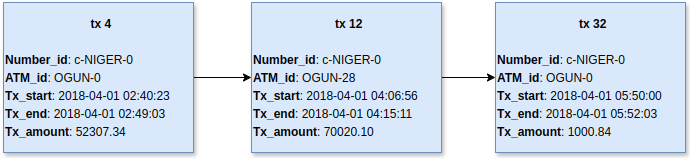
\includegraphics[scale = 0.45]{images/3-Engine/subgraph.png}
    \caption{Subgraph \texttt{edges} linked list of transactions of the \texttt{c-NIGER-0} card filter example}
    \label{img:pipeline-subgraph}
\end{figure}

\paragraph{Operations}
The operations related with the inner filter data structure are the following:

\begin{itemize}
    \item \texttt{NewGraph()}: Creates a new \texttt{Graph} data structure. This is done on the creation of the filter.
    
    \item \texttt{AddAtEnd(e Edge)}: Adds a new edge. Appends a new edge at the end of the list \texttt{edges} and updates the \texttt{last\_timestamp} variable with the \texttt{Tx\_end} time of the new added edge. This operation is done whenever a new transaction edge of the associated card arrives to the filter.
    
    \item \texttt{Update(timestamp time.Time)}: Given a certain datetime, it updates the subgraph, starting from the first edge of the \texttt{edges} list, by eliminating those that are outdated with respect to this datetime. An edge $e$ is outdated  whenever its time difference with respect to the incoming timestamp is greater than the fixed window time constant \texttt{timeTxThreshold}. That is, whenever: $$timestamp - e.Tx\_end \geq timeTxThreshold$$
    This operation is done in two situations:
    \begin{itemize}
        \item $edge \in filter$ ($filter.Number\_id = edge.Number\_id$) Whenever the transaction edge belongs to our filter. Before performing the \texttt{AddAtEnd} operation we perform the \texttt{Update} operation with the timestamp of the new transaction. This ensures that only transactions inside the fixed window of time are considered to do associations for fraud detection. 
        \item $edge \notin filter$ ($filter.Number\_id\ \neq edge.Number\_id$) Whenever a transaction edge passes through our filter but it does not belong to it. We take its timestamp as the \texttt{timestamp} parameter of the \texttt{Update} operation.
    \end{itemize}
    
    \item \texttt{CheckFilterTimeout(timestamp time.Time) bool}: Given a timestamp, it tests if the filter has to be deleted due to a long time of detected \textit{inactivity}. A filter is decided to be deleted if the time difference between the last edge of the subgraph (saved in the \texttt{last\_timestamp} variable) and the incoming \texttt{timestamp} is greater than the fixed \texttt{timeFilterThreshold} time constant: $$timestamp - last\_timestamp \geq timeFilterThreshold$$
    This operation is only performed whenever $edge \notin filter$, taking its timestamp as our parameter, in particular before the \texttt{Update} operation, since in the case the filter needs to be deleted, the \texttt{Update} operation will no longer have to be performed.

    \item \texttt{CheckFraud(new\_e Edge) bool}: \textcolor{blue}{TODO: This is the temporal approximate approach} So far, it is assumed that the current volatile subgraph of the filter is correct (in the sense that it is considered to be free of anomalous transactions). For the moment, only the kind of fraud explained at section \ref{fraud-pattern-1} is checked. \textcolor{blue}{More specifically, the way to perform the check is ONLY between the new incoming edge belonging to the filter \texttt{new\_e} and the last edge that was added to the volatile subgraph. And if, this kind of fraud pattern is matched then an alert is output and this last edge is considered to be anomalous and therefore it is not added to the volatile subgraph of the filter}. 
    
\end{itemize}

With these operations, a summary of the algorithmic behavior of a filter can be seen in the flow diagram on Figure \ref{diag:filter-flow}.

% TODO: Poner ejemplos con dibujitos
% TODO: Diagrama de flujo / casos, para aclarar bien los diferentes casos y qué hago en cada situación
\begin{figure}[H]
    \centering
    \begin{tikzpicture}[node distance=2cm]
\node (start) [startstop] {New Filter (Edge e)};
\node (creation) [process, below of=start] {
    \texttt{NewGraph()}\\
    \texttt{AddAtEnd(e)}
};
\node (while) [process, below of=creation]{in: new edge};
\node (edgeInFilter) [decision, below of=while, yshift=-1cm] {$edge \in filter$};

\node (edgeFilterYes) [process, right of=edgeInFilter, xshift=3cm, text width=4cm] {
    \texttt{Update(edge.Tx\_start)}
    \texttt{AddAtEnd(edge)}
    \texttt{CheckFraud()}
};
\node (filterTimeout) [decision, below of=edgeInFilter, yshift=-2.5cm, text width=3.1cm] {\texttt{CheckFilterTimeout\\(edge.Tx\_start)}};
\node (filterTimeoutNo) [process, right of=filterTimeout, xshift=7cm, text width=4cm] {
    \texttt{Update(edge.Tx\_start)}
};
\node (stop) [startstop, below of=filterTimeout, yshift=-2cm] {Stop};

\draw [arrow] (start) --  (creation);
\draw [arrow] (creation) -- (while);
\draw [arrow] (while) -- node[anchor=east] {edge} (edgeInFilter);
\draw [arrow] (edgeFilterYes) |- (while);
\draw [arrow] (edgeInFilter) -- node[anchor=south] {yes} (edgeFilterYes);
\draw [arrow] (edgeInFilter) -- node[anchor=east] {no} (filterTimeout);
\draw [arrow] (filterTimeout) -- node[anchor=south] {no} (filterTimeoutNo);
\draw [arrow] (filterTimeoutNo) |- (while);
\draw [arrow] (filterTimeout) -- node[anchor=east] {yes} (stop);
\end{tikzpicture}

    \caption{Filter flow diagram}
    \label{diag:filter-flow}
\end{figure}

\paragraph{Considerations}
\begin{itemize}
    \item So far, the way to perform the \texttt{Update} and the \texttt{CheckFilterTimeout} operations could be described as a kind of \textit{filter lazy updating}, since only the filters located before the filter to which the transaction edge finally belongs are updated with the timestamp of that edge. Whereas the filters located after this filter will not be updated with this timestamp. The cause of this is that once the edge is filtered to its corresponding filter, it \textit{sinks} into it, and therefore it is not propagated to the consecutive filters. See the case on Figure \ref{img:pipeline-update-issue}, where if a transaction edge was to belong to the filter F3, then only the filters F1, F2 and F3 will be updated accordingly to the timestamp of this edge, whereas the filter F4 will not be updated in this case.
    \begin{figure}[H]
        \centering
        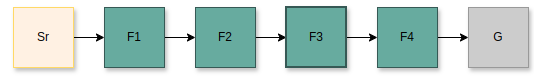
\includegraphics[scale = 0.45]{images/3-Engine/update-issue.png}
        \caption{Pipeline \textit{filter lazy updating} example}
        \label{img:pipeline-update-issue}
    \end{figure}
    However, this is not necessarily a problem. The reason is that the filter will perform these operations later in the future. Note that in the case that the edge belongs to the filter, the \texttt{Update} operation will be performed just before doing the \texttt{AddAtEnd} operation as it was already mentioned in the description of the \texttt{Update} operation. \textcolor{red}{Note that to avoid this "problem" another approach could be done like doing a timestamp channel or passing all the edges until the end of the pipeline.} 
    \item Due to the nature of the management of the filter's lifetime and subgraph updating, it can be the case that our filter subgraph is empty, although the filter is still alive. We can arrive to this situation by having deleted all the edges of the filter subgraph since they were outdated, but still the \texttt{timeFilterThreshold} time has not yet passed. However, thanks to the saved \texttt{last\_timestamp} variable we do not need to save the last edge or do anything but comparing the incoming timestamp with this 
    \texttt{last\_timestamp} variable (calling the function \texttt{CheckFilterTimeout()}).
\end{itemize}
% - last_timestamp parameter helps avoid having to save the last edge completely. The case of the subgraph being empty % but the filter still be active case

% TODO: Tests!!!!
% 1. AddAtEnd -> no añadir...
% 2. Update   -> añadir?
% 3. Filter timeout  -> añadir? (*) igual sólo añadir este, pues es más completo e incluye a los anteriores


\section{Experiments Notes}

\subsubsection{E2: Continuous delivery of results in a high loaded scenario}

Do not consider the real-time simulation, by omitting the transaction timestamps in the sense that we do not consider them to simulate a real case scenario where each transaction arrives to the system at the time indicated by its timestamp. 
Instead all the stream comes (ordered by timestamp) but directly (almost) at the same time to the system. With this approach:
\begin{itemize}
  \item \textbf{No real case simulation}
  \item \textbf{Measure the load the system can take}: for the different system variations given a same stream.
  \item \textbf{Diefficiency metrics}: since time arrival of the transactions to the system is now ignored, and all the transactions come one after the other, a result to be produced do not need to wait for the real timestamp of the transaction. Therefore, we could see the differences in continuously delivering results of the different systems under the same input stream load (more clear than before).
\end{itemize}

\begin{tcolorbox}[colframe=red!75]
\textcolor{red}{\textbf{IMPORTANT: WHAT DO WE WANT TO TEST?\\}}
Definition of the objectives of the experiments:
\begin{itemize}
    \item See and compare the behavior of the system(s) with different streams (different number of cards, greater or smaller size of the bank - and therefore its database). \\
    \textcolor{teal}{Objective: see that the dp approach is better to handle bigger stream sizes.}
    \begin{itemize}
        \item Continuous delivery of results comparison (diefficiency metrics).
        \item Total execution time needed to process the full stream.
        \item Maximum endurance capacity of the system(s) -- until which size of stream can the system work without crashing (\textit{Hasta donde podemos llegar a aguantar con nuestro sistema. Capacidad de carga máxima.})
    \end{itemize}
\end{itemize}
\end{tcolorbox}

\paragraph{Problems derived:\\}
\begin{itemize}
    \item \textbf{The load we are simulating is way higher than real (of course higher than for the real time approach)}
    \item \textbf{The reading of the input can be our bottleneck}: Try to find the fastest way to deal with it (described in \ref{input-reading}).    
\end{itemize}

\textbf{What we do then?}
$\rightarrow$ Try both kinds of experiments. 
For the first:
\begin{itemize}
    \item Document what I have and explain what I have seen so far.
    \item Continue running some more to see if I can see more differences. With more transactions and stream load.
    \item Try to scale to the millisecond/nanosecond timestamp precision. See if I can avoid losing alerts.
\end{itemize}
For the second:
--- START THEM, following the variations in the notebook (already explained)---

\begin{itemize}
  \item Q2: Behavior of the different system variations on a high loaded transaction stream scenario.
  \item R2: Not real time simulation. Direct transaction stream input supply. Comparison of the continuous delivery of results of the different systems variations (diefficiency metrics).
\end{itemize}

\subsubsection{Small bank size \& small transaction stream}

\paragraph{1-core\\}

\ad{Hay que explicar bien los resultados que se enseñan en cada grafica y lo que representan además de las conclusiones que permiten sacar.}

Results for executions with 1-core:

\begin{figure}[H]
  \centering
  \includegraphics[scale = 0.5]{images/4-Experiments/E2/fixedcores/1c/traces.png}
  \caption{Alerts trace in time (s) - 1 core}
\end{figure}

\begin{figure}[H]
  \centering
  \includegraphics[scale = 0.5]{images/4-Experiments/E2/fixedcores/1c/execTime.png}
  \caption{Execution time (s) - 1 core}
\end{figure}

\begin{figure}[H]
  \centering
  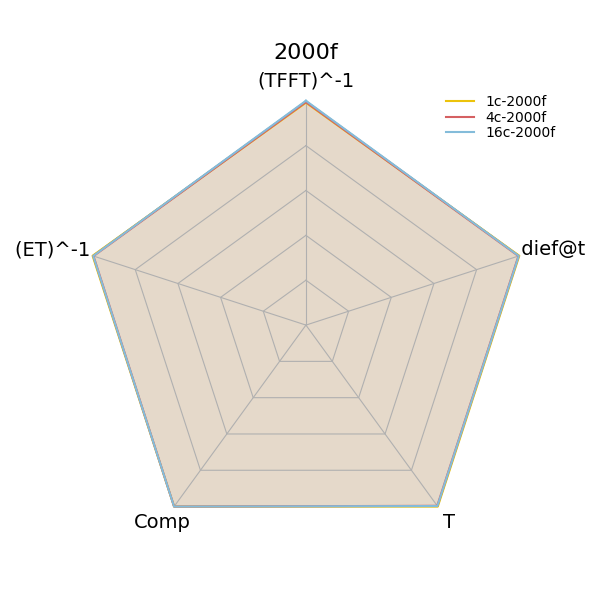
\includegraphics[scale = 0.5]{images/4-Experiments/E2/fixedcores/1c/radar-dieft.png}
  \caption{\texttt{dieft} radar - 1 core}
\end{figure}

\begin{figure}[H]
  \centering
  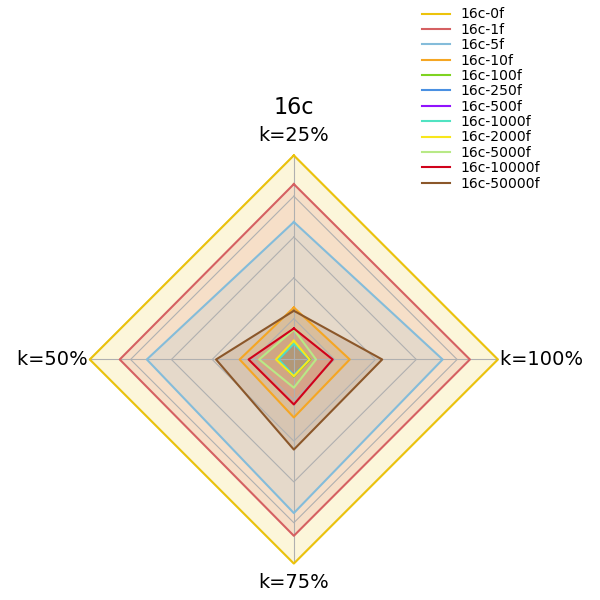
\includegraphics[scale = 0.5]{images/4-Experiments/E2/fixedcores/1c/radar-diefk.png}
  \caption{\texttt{diefk} radar - 1 core}
\end{figure}

\textcolor{red}{TODO: Put table for not graphical results gathered in the dieffpy-out.txt file...}

\paragraph{4-cores\\}

Results for executions with 4-core:

\begin{figure}[H]
  \centering
  \includegraphics[scale = 0.5]{images/4-Experiments/E2/fixedcores/4c/traces.png}
  \caption{Alerts trace in time (s) - 4 core}
\end{figure}

\paragraph{8-cores\\}

Results for executions with 8-core:

\begin{figure}[H]
  \centering
  \includegraphics[scale = 0.5]{images/4-Experiments/E2/fixedcores/8c/traces.png}
  \caption{Alerts trace in time (s) - 8 core}
\end{figure}

\paragraph{16-cores\\}

Results for executions with 16-core:

\begin{figure}[H]
  \centering
  \includegraphics[scale = 0.5]{images/4-Experiments/E2/fixedcores/16c/traces.png}
  \caption{Alerts trace in time (s) - 16 core}
\end{figure}

\textcolor{red}{NOTE: Almost no difference when variating the number of cores!!!!}

\begin{figure}[H]
  \centering
  \begin{subfigure}[b]{0.45\textwidth}
    \centering
    \includegraphics[scale=0.6]{images/4-Experiments/E2/fixedcores/1c/execTime.png}
    \caption{Execution time (s) - 1 core}
  \end{subfigure}
  \hfill
  \begin{subfigure}[b]{0.45\textwidth}
    \centering
    \includegraphics[scale=0.6]{images/4-Experiments/E2/fixedcores/4c/execTime.png}
    \caption{Execution time (s) - 4 core}
  \end{subfigure}
  \\
  \begin{subfigure}[b]{0.45\textwidth}
    \centering
    \includegraphics[scale=0.6]{images/4-Experiments/E2/fixedcores/8c/execTime.png}
    \caption{Execution time (s) - 8 core}
  \end{subfigure}
  \hfill
  \begin{subfigure}[b]{0.45\textwidth}
    \centering
    \includegraphics[scale=0.6]{images/4-Experiments/E2/fixedcores/16c/execTime.png}
    \caption{Execution time (s) - 16 core}
  \end{subfigure}
  \caption{Execution times for different core configurations.}
  \label{fig:execution-times}
\end{figure}


\textcolor{blue}{
Some observations:
\begin{itemize}
    \item Differences between  more or less cores visible specially for a fixed big number of filters (see plots of fixed number of filters) -> TODO
    \item More filters imply more overhead specially when number of cores is low.
\end{itemize}
}

\paragraph{Transaction stream - medium\\}

\begin{itemize}
  \item $\texttt{NUM\_DAYS} = 60$
  \item $\texttt{anomalous\_ratio} = 0.02\ (2\%)$ 
\end{itemize}

This setup gives us a transaction stream of 
\begin{itemize}
  \item $\texttt{total\_tx} = 80744$
  \item $\texttt{regular\_tx} = 79005$
  \item $\texttt{anomalous\_tx} = 1739$
\end{itemize}

\paragraph{Transaction stream - big\\}

\begin{itemize}
  \item $\texttt{NUM\_DAYS} = 120$
  \item $\texttt{anomalous\_ratio} = 0.02\ (2\%)$ 
\end{itemize}

This setup gives us a transaction stream of 
\begin{itemize}
  \item $\texttt{total\_tx} = 160750$
  \item $\texttt{regular\_tx} = 157756$
  \item $\texttt{anomalous\_tx} = 2994$
\end{itemize}

\textcolor{blue}{NOTE: only 5 runs each experiments instead of 10! - large execution time...}

\rule{\textwidth}{0.4pt} 
\textcolor{red}{$\rightarrow$ Issue: Connection timeout\\}
In the cases: 
\begin{itemize}
    \item 1c: $\ge 200f$
    \item 2c: $\ge 1000f$
\end{itemize}

Possible fixes:
\begin{itemize}
    \item (Optimization of the query... introducing indexing!)
    \item Increase the timeout
    \item Set a maximum connection pool size... Note that it may be needed for later experiments...
    Since we may not be able to open more than $x$ connections/sessions in parallel with the Neo4j gdb. Then we have 2 options:
    \begin{itemize}
        \item Limit the maximum number of filters based on this max limit on the number of parallel connections/sessions.
        \item Do not limit the maximum number of filters, but instead create a pool of connections.
    \end{itemize}
    \begin{enumerate}
        \item So far $\rightarrow$ Try to fix limiting the maximum timeout and limit the number of filters (with the idea that each filter has a permanent open session - instead of requesting a session from a pool of connections to a certain process manager of sessions every time it needs to query... - I think it is more clean and easy, and for the purposes of what we are doing to have a permanent open session per filter. So that:
        \begin{itemize}
            \item Easier to manage (apparently no limit on the number of parallel sessions - so no problem)
            \item We need to do a retry process - so that whenever the timeout exceeds it can try again without producing an error - and/or increase the timeout limit.
            \item Finally note that this problem is going to appear whenever we have many open threads connected in a high loaded scenario tested on a low-resource variant of the system (with few/low number of cores). And that, for a real scenario this is not going to be the case since the system will be expected to be way less loaded.
        \end{itemize}
    \end{enumerate}
\end{itemize}

\textcolor{green}{$\rightarrow$ Partial fix so far: increase the timeout of a transaction at the driver level to 1h: "config.MaxTransactionRetryTime = 1 * time.Hour"\\}

\textcolor{blue}{Some details about our Neo4j VM:
\begin{itemize}
    \item 4 cores and 20GB of RAM
    \item No limit on the number of parallel sessions. However it seems that by default there is a limit on the number of parallel transactions to 1000.
\end{itemize}
}

\subsection*{E2: Evaluation in a Real-World Stress Scenario}


E1: Mean Response Time

\begin{itemize}
  \item Q1: How much it takes for the system to emit the alerts from the moment the anomalous transaction was produced.
  \item R1: Real time simulation. Measuring the mean response time from the start of the transaction of the detected anomalous scenario until the alert is emitted by the system.
\end{itemize}


Note that, because of the way we did the transaction generator (coming from wisabi database client's behavior), the average number of transactions per day per card is $\sim1$, and therefore to be able to generate a transaction set with anomalous situations more close to reality, a reasonable time interval size for the generated transaction stream would be having $T$ around some weeks or month(s).

\subsubsection{E1: Mean Response Time}

\textbf{Real time-event stream simulation\\}
Since we do not have the material time to run each experiment for a interval time $T$ of some weeks or a month the idea is to do time scaling of the time event stream. We take the stream of a certain time interval size $T$ and map it into a smaller time interval
$T'$ where $T' << T$. Then, we do a real-time event simulation, providing the events of the input stream to the system at the times they actually occur (in reality possibly with a small certain delay!) using their timestamps.

\begin{itemize}
  \item \textbf{Shorter experimental time}: Reduced time to test the system behavior. Instead of $T$, only $T'$ time to test it. 
  \item \textbf{Stress testing - Graph database size - amount of filters' subgraphs}: We do not test the system under a real-case scenario considering its number of cards $c$, instead we are testing it under a higher load to what it would correspond, but having $c$ cards, and therefore $c$ filter's subgraph. The benefit is that we do not need to have such a big graph database.
\end{itemize}

The consequences for the experiments and metrics:

\begin{itemize}
  \item \textbf{Diefficiency metrics} (continuous delivery of results): If we give the input stream to the system respecting the temporal timestamps, note that no matter the system characteristics, that a result (an alert in our case), will not be possible to be produced until the event causing it arrives to the system. Therefore the emission of events is expected to be really similar in this case, for any system variation. Only in the case when the stream load is high enough we expect to see some differences?? \textcolor{orange}{$\rightarrow$ HABRÁ QUE IR VIÉNDOLO...}
  \item \textbf{Response time}: having in mind the previous considerations, we think in measuring the possible differences of behavior of the different system capabilities in terms of the mean response time. The mean response time (\texttt{mrt}) would be the average time that the system spends since it receives the transactions involved in an alert until the time it emits the alert.
\end{itemize}

\textcolor{red}{Problems derived to pay attention to}:
\begin{itemize}
  \item Shrinking the timestamps to a smaller time interval, produces the emergence of not real fraud patterns that before did not exist due to their real and "correct" larger time distance. Example:
  \begin{itemize}
  \item Consider the original size of the time interval of the input stream $T=120h$ (5 days) and $T'=24h$.
  \item Consider two consecutive regular transactions of a certain client performed in two different ATMs \texttt{ATM-x} and \texttt{ATM-y} with \texttt{t\_min}$=8$h (minimum time difference to traverse the distance from \texttt{ATM-x} to \texttt{ATM-y}) and \texttt{t\_diff}$=24$h (time difference between the first and the second transaction). 
  \item \textcolor{red}{$\rightarrow$ Note that with the scaling the time difference \texttt{t\_diff} would be of 5 times less, that is, $\texttt{t\_diff}=4.8h$. Therefore this will make $\texttt{t\_diff'}=4.8h < \texttt{t\_min}=8h$}.
  \end{itemize}
  \item $\rightarrow$ (*) Solution A: \textbf{introduce the scaling factor as a input parameter} and consider it also for the fraud checking so to properly \textbf{scale the $\texttt{t\_min}$ variable} ($\texttt{t\_min}=8h \rightarrow \texttt{t\_min'}=\frac{8}{5}h=1.6h$) and therefore: 
  \begin{itemize}
    \item Before scaling: $\texttt{t\_diff}=24h > \texttt{t\_min}=8h$.
    \item After scaling (scale factor $=\frac{1}{5}$): $\texttt{t\_diff}=24*\frac{1}{5}=4.8h > \texttt{t\_min}=8*\frac{1}{5}=1.6h$.
  \end{itemize}
  \item $\rightarrow$ Solution B: conserve the original timestamps, and consider the mapped-reduced timestamps for simulating the arrival times of the transactions into the system while taking the original timestamps for the checking of the frauds.
\end{itemize}

\begin{tcolorbox}[colframe=red!75]
\textcolor{red}{\textbf{IMPORTANT: WHAT DO WE WANT TO TEST?\\}}
Definition of the objectives of the experiments:
\begin{itemize}
    \item See and compare the behavior of the system(s) with different streams (different number of cards, greater or smaller size of the bank - and therefore its database). \\
    \begin{itemize}
        \item Alert/result response time comparison. \textbf{Continuous delivery of results (diefficiency metrics) does not make sense!}. With the objective to see that we can see lower response time in the case of the dp versions.
    \end{itemize}
\end{itemize}
\end{tcolorbox}

\ad{Esto tiene que ir al principio de la sección de experimentos, tienes que explicar "con palabras" qué es lo que quieres probra y luego cómo lo haces.}

\paragraph{Problems derived:\\}
\begin{itemize}
    \item \textbf{Continuous delivery of results comparison does not make sense.} $\rightarrow$ In a real time simulation, for any system, results can only be emitted whenever the corresponding anomalous transaction $a_i$ reaches the system. That happens at the same time $t_i$ for both approaches when the input stream is simulated at real time, meaning that the result corresponding to the anomalous transaction $a_i$ can not be emitted in any case before time $t_i$. Therefore, the difference in time delivery of this result between the different approaches is not expected to be high unless we make the systems to be loaded enough. \textbf{Therefore, for small sized banks this does not really make sense...}
    \item \textbf{Losing of alerts}: Due to scaling we are losing alerts since we have seconds precision. We will have to scale to the millisecond or nanosecond the timestamps to possibly do not loose those alerts, due to time scaling precision.
    \item \textbf{Although scaling, the load we are simulating is higher than real... - like for the not real time approach}
\end{itemize}

\subsubsection{Initial experiments}

\textit{Small} initial graph database (gdb) size:
\begin{itemize}
  \item $|ATM| = 50$
  \item $|Card| = 2000$
\end{itemize}

Transaction stream:
\begin{itemize}
  \item $\texttt{NUM\_DAYS} = 30$
  \item $\texttt{anomalous\_ratio} = 0.02\ (2\%)$ 
\end{itemize}

This setup gives us a transaction stream of 
\begin{itemize}
  \item $\texttt{total\_tx} = 39959$
  \item $\texttt{regular\_tx} = 39508$
  \item $\texttt{anomalous\_tx} = 451$ -- note that this is actually a $1\%$.
\end{itemize}

\begin{table}[H]
\centering
\begin{tabular}{|c|c|c|c|c|c|}
  \hline
  Execution & Scaled   & Num. cards/filter& Num. cores & Num. alerts & Time(s) \\ \hline
  NRT & No & Baseline (all) & 1 & 462 & 44.88 \\ \hline
  RT  & 1h & Baseline (all) & 1 & 447 & 3601.65\\ \hline
  RT  & 1h & 500 (4 filters) & 4 & 447 & 3603.25\\ \hline
  RT  & 1h & 200 (10 filters) & 10 & 447 & 3602.71\\ \hline
  RT  & 6h & Baseline (all) & 1 & 459 & 21606.11 \\ \hline
  RT  & 6h & 500 (4 filters) & 4 & 459 & 21611.75 \\ \hline
  RT  & 12h & Baseline (all) & 1 & 461 & 43211.95 \\ \hline
\end{tabular}
\caption{Different experimental setups results}
\label{table:small-results}
\end{table}

Some nomenclature:
\begin{itemize}
  \item NRT: Not Real Time execution
  \item RT: Real Time execution
\end{itemize}

Some results:

\paragraph{1h scaling\\}

\ad{Los captions de las figuras tienen que ser autocontenidos.}


\begin{figure}[H]
  \centering
  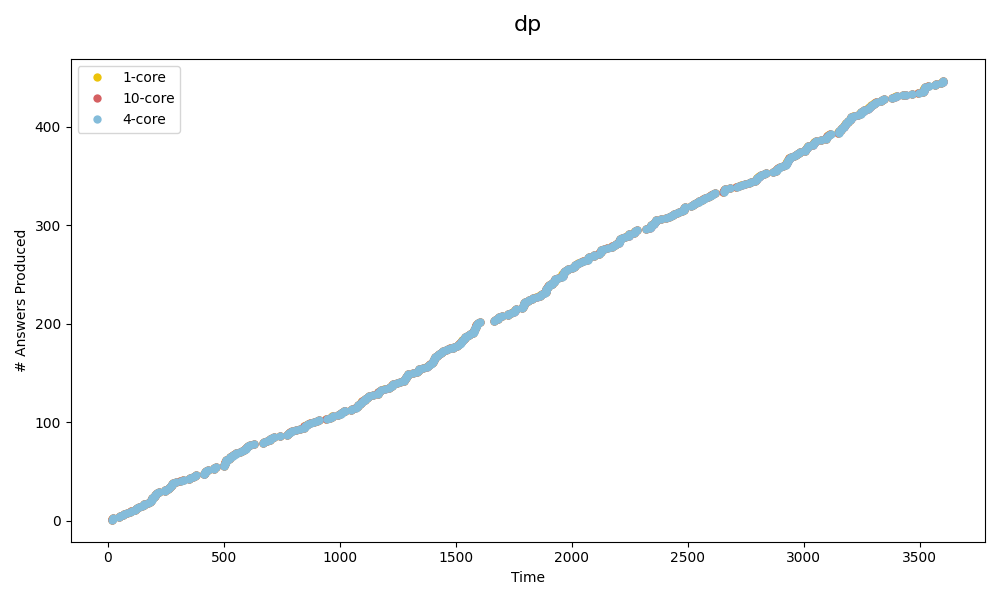
\includegraphics[scale = 0.5]{images/4-Experiments/traces-1h.png}
  \caption{Trace 1h}
\end{figure}

Only for the first 10 results (alerts):
\begin{figure}[H]
  \centering
  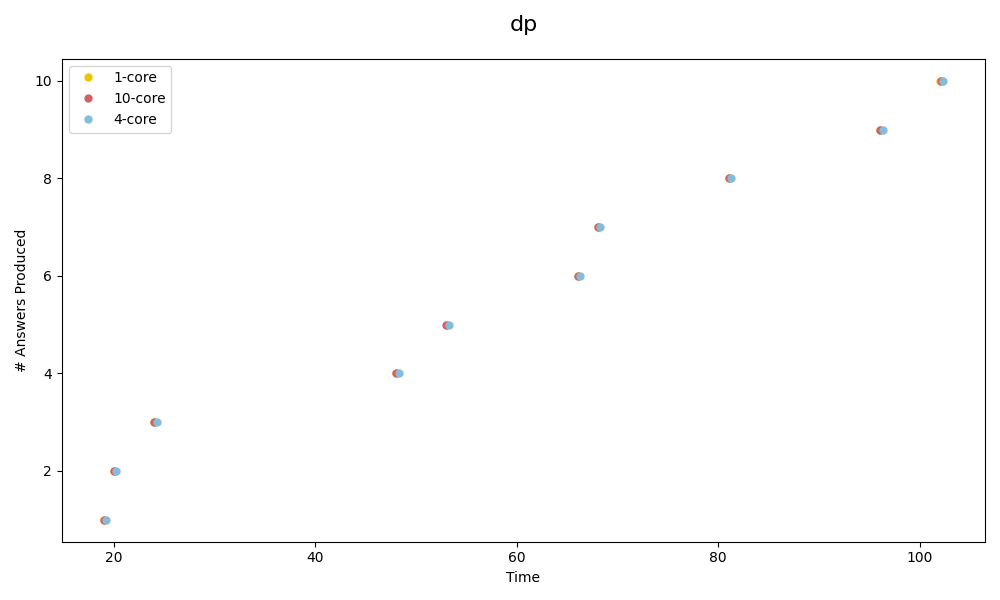
\includegraphics[scale = 0.5]{images/4-Experiments/traces-1h-10.png}
  \caption{Trace 1h - first 10 alerts}
\end{figure}

\paragraph{6h scaling\\}

We do not see any difference in the behavior between the baseline with 1 filter and 1 core approach (\texttt{RT-6h-1c-1f}) and the approach with 4 filters and 4 cores (\texttt{RT-6h-4c-4f}). 

\textbf{WHY?} $\rightarrow$ a possible reason is that results can only be emitted whenever the corresponding anomalous transaction $a_i$ reaches the system. That happens at the same time $t_i$ for both approaches when the input stream is simulated at real time, meaning that the result corresponding to the anomalous transaction $a_i$ can not be emitted in any case before time $t_i$. Therefore, the difference in time delivery of this result between the different approaches is not expected to be high unless we make the systems to be loaded enough.

\subsection{Definitive Experiments}

$\rightarrow$ We set the worker stream reading by chunks, with chunk size of $10^2$.\\

The setups of the experiments that we are going to do are:
\begin{itemize}
  \item Fix different bank sizes (small, $+\frac{1}{4}$, $+\frac{2}{4}$, $+\frac{3}{4}$, the biggest possible size).
  \begin{itemize}
    \item For each, generate different stream sizes.
    \begin{itemize}
      \item Compare different system variations in the number of cores and number of filters.
    \end{itemize}
  \end{itemize}
\end{itemize}

\begin{table}[H]
\centering
\begin{tabular}{|c|c|c|c|}
\hline
Bank Size & \# Cards & \# ATMs & Stream Size (\# tx) \\ \hline
Small     & 2000     & 50 (45 internal - 5 interbank)     & 39959 - small       \\ \hline
Small     & 2000     & 50 (45 internal - 5 interbank)      & 80744 - medium      \\ \hline
Small     & 2000     & 50 (45 internal - 5 interbank)     & 160750 - big        \\ \hline
Medium    & 500000   & 1000 (900 internal - 100 interbank)   &                     \\ \hline
          &          &         &                     \\ \hline
          &          &         &                     \\ \hline
Big       &          &         &                     \\ \hline
Big       &          &         &                     \\ \hline
Big       &          &         &                     \\ \hline
\end{tabular}
\end{table}

\subsubsection{Bank size: Initial - Small}

\begin{itemize}
  \item $|ATM| = 50$
  \item $|Card| = 2000$
\end{itemize}

\paragraph{Transaction stream - small\\}

\begin{itemize}
  \item $\texttt{NUM\_DAYS} = 30$
  \item $\texttt{anomalous\_ratio} = 0.02\ (2\%)$ 
\end{itemize}

This setup gives us a transaction stream of 
\begin{itemize}
  \item $\texttt{total\_tx} = 39959$
  \item $\texttt{regular\_tx} = 39508$
  \item $\texttt{anomalous\_tx} = 451$ -- note that this is actually a $1\%$.
\end{itemize}

For different core variations, we are going to try different combinations of the system in terms
of the number of the maximum number of cards per filter, that consequently will produce an inverse variation in the number of filters of the system.

\begin{table}[H]
  \renewcommand{\arraystretch}{1.5} % control row height
  \centering
  \begin{tabular}{|c|c|}
  \hline
  \# cards per filter & \# filters \\ \hline
  2000   &   1     \\ \hline
  1000   &   2     \\ \hline
  400 &   5     \\ \hline
  200  &   10     \\ \hline
  100 &   20    \\ \hline
  50  &   40    \\ \hline
  20  &   100    \\ \hline
  10  &   200    \\ \hline
  4  &   500    \\ \hline
  2  &   1000    \\ \hline
  1  &   2000    \\ \hline
  \end{tabular}
\end{table}

\begin{itemize}
  \item \# of times / runs each job $=10$.
  \item Maximum RAM limited to 16GB.
\end{itemize}

\subsection{E1: Mean Response Time}

\begin{itemize}
  \item Q1: How much it takes for the system to emit the alerts from the moment the anomalous transaction was produced.
  \item R1: Real time simulation. Measuring the mean response time from the start of the transaction of the detected anomalous scenario until the alert is emitted by the system.
\end{itemize}

Setting up the experiments:

\begin{itemize}
    \item Scaling issue: \textcolor{green}{- Fixed - scaled at the level of the $\mu$s}
\end{itemize}

\subsubsection{Small bank size \& small transaction stream}

\begin{itemize}
    \item Scaling to 600s (10 minutes) $\rightarrow$ no losing of alerts (462).
\end{itemize}

\textcolor{blue}{
My doubts on these experiments
\begin{itemize}
    \item Results = Checks: same issue as with the alerts, a same check(tx1,tx2) on a card can not be performed until the tx2 reaches the system, which is the same simulated time on any system.
    \item For a small bank size, as the simulation tends to be closer to reality (lower scaling), 
    then the system has lower overhead and the differences between the different variations will be almost negligible. Also the time needed to perform these simulations increases.
    \item However, on the contrary, when the scaling is high, then the simulation is farther from reality, making the system to be more loaded than in a real case scenario, reaching a point that the experiment will be almost the same as E2 (reading the transaction stream input directly without any real-time simulation).
    \item To have a "real-time" simulation in which differences between the systems can be observed we will need to simulate a big bank, which is able to provide a dense/big stream, which intuitively, even more if the stream is scaled, the simulation will be almost like reading the stream directly from the input like without any "real-time" simulation, like in the case of the E2 experiments. 
\end{itemize}
}

\textcolor{orange}{
Proposals:
\begin{itemize}
    \item Do more variations on the stream size and bank database size for the E2 experiments.
    \begin{itemize}
        \item Incrementing the database size, is expected to increase the overhead due to the greater number of cards and the latency to query the stable bank database.
        \item Increasing the stream size...?
    \end{itemize}
    \item On the E2 experiments measure and compare the response time for providing an alert (the time since the last transaction producing the alert happened until the time the system emits out that alert). \textbf{But focusing only on the alerts and not on all the checks, I think it is sufficient to compare only on the alerts.} Also measuring on the checks will introduce an overhead on the needed message passing from the filters to the sink to do all this gathering on these times, whereas with the alerts it is minimal since they are already sent to the Sink stage.
\end{itemize}
}

Some experiments that were tested:

\begin{itemize}
    \item Scaled small bank data stream of 30 days to 10 minutes.
    \item Tested for these combinations:
    \begin{table}[H]
      \renewcommand{\arraystretch}{1.5} % control row height
      \centering
      \begin{tabular}{|c|c|}
      \hline
      \# cores & \# filters \\ \hline
      1        & 1  \\ \hline
      4        & 40  \\ \hline
      16       & 2000  \\ \hline
      \end{tabular}
    \end{table}
\end{itemize}

\rule{\textwidth}{0.4pt} 

\subsection{Update: Recording all the checks}

\subsection{How to measure MRT}\label{exp-measuring-mrt}

To show the continuous delivery of results of the system, for testing purposes, instead of only recording the alerts (positive fraud checks) in the Sink, we are now going to be recording all the check results whether they are positive (alerts) or negative.\\
How we do this?\\
Measurement options:
\begin{itemize}
    \item Measure the \texttt{time.End} of the check on the Sink. As with the alerts is the time it takes for the system to emit the result.
    \item Measure the \texttt{time.End} of the check on the Filter. It could be argued that the alerts (which are the unique results that in reality get out of the system) could be directly be sent from the Filters and not from the Sink, saving the time they need to travel to the Sink inside the system. Anyway they will need to travel to the Sink to be registered on the bank system but the alert to the user could be directly sent faster from the Filters.
\end{itemize}

So far:
\begin{itemize}
    \item Measurement: done at the Sink.
    \item Register of the results at the Sink and sent all (positive and negative) through a unique channel from each Filter to the Sink (we reuse the \texttt{alert} channel).
\end{itemize}

Some experiments were done to inspect whether there was a significant difference on the measurement position. In particular, we measured the response time of each of the checks both in the Filter and in the Sink, to finally obtain the mean response metrics times of both approaches. In the table \ref{tab:response-time-measurement-comparison} we show the mean response time metric in ms measured at the Sink (\texttt{mrt-Sink}) and the difference of this measurement on average with respect to the measurement done in the Filter in ms (\texttt{mrt-difference}).

Note that each of this experiments were done running in not-real-time, with the small bank size, and the \texttt{30-0.02} stream. Each of the experiments were run 10 times... 16GB RAM...

\textcolor{blue}{As it can be observe the differences are negligible, and therefore for simplicity, and to maintain the "philosophy" of the dynamic pipeline, we decided to keep the measurement of the response times of the checks on the Sink stage.}

\textcolor{red}{Note that, measuring in the Filter would imply assuming that the alerts had to be sent from there, to be realistic to where we are measuring.}
\textcolor{red}{Note that: measuring all the results and not only the alerts imply unnecesarily overloading the system, since only sending the alerts to the Sink should be enough for the purposes of our application. However, due to experimental purposes we are forced to send/measure all the checks, in order to be able to compare the continuous delivery of results of all the system configurations/variations}.

\begin{table}[H]
\centering
\begin{tabular}{|c|c|c|c|}
\hline
\# filters & \# cores & \begin{tabular}[c]{@{}c@{}}mrt-Sink\end{tabular} & \begin{tabular}[c]{@{}c@{}}mrt-difference\end{tabular} \\ \hline
1          & 1        & 24899.103                                                         & 0.071                                                                          \\ \hline
1          & 4        & 24077.638                                                         & 0.041                                                                          \\ \hline
1          & 16       & 22302.060                                                         & 0.016                                                                          \\ \hline
40         & 1        & 8852.990                                                          & 0.195                                                                          \\ \hline
40         & 4        & 8012.537                                                          & 0.065                                                                          \\ \hline
40         & 16       & 8241.212                                                          & 0.040                                                                          \\ \hline
2000       & 1        & 13949.781                                                         & 2.229                                                                          \\ \hline
2000       & 4        & 10464.550                                                         & 0.847                                                                          \\ \hline
2000       & 16       & 7982.963                                                          & 0.052                                                                          \\ \hline
\end{tabular}
\caption{Comparison of the response time measurement positions with different system configurations}
\label{tab:response-time-measurement-comparison}
\end{table}

\subsubsection{Bank size: Medium}

\textcolor{red}{For these experiments, to generate the stream of tx, we needed to simplify this process in order to be able to generate a stream in a feasible amount of time. In particular we used the simplifed version of the \texttt{txGenerator.py}: \texttt{txGenerator-simplified.py} $\rightarrow$ with a random ATM-subset instead of a closest to client ATM-subset. Also variation on the transaction distribution times.}


\begin{itemize}
  \item $|ATM| = 1000$
  \item $|Card| = 500000$
\end{itemize}

\begin{table}[H]
  \renewcommand{\arraystretch}{1.5} % control row height
  \centering
  \begin{tabular}{|c|c|}
  \hline
  \# cards per filter & \# filters \\ \hline
  500000   &   1     \\ \hline
  100000   &   5     \\ \hline
  50000 &   10     \\ \hline
  5000  &   100     \\ \hline
  2000 &   250    \\ \hline
  1000  &   500    \\ \hline
  500  &   1000    \\ \hline
  250  &   2000    \\ \hline
  100  &   5000    \\ \hline
  50  &   10000    \\ \hline
  10  &   50000    \\ \hline
  \end{tabular}
\end{table}

\paragraph{Transaction stream - small\\}


\begin{itemize}
  \item $\texttt{NUM\_DAYS} = 15$
  \item $\texttt{anomalous\_ratio} = 0.03\ (3\%)$ 
\end{itemize}

This setup gives us a transaction stream of 
\begin{itemize}
  \item $\texttt{total\_tx} = 4856573$
  \item $\texttt{regular\_tx} = 4805920$
  \item $\texttt{anomalous\_tx} = 50653$
\end{itemize}

First run:
\begin{itemize}
    \item 16GB RAM
    \item 16 cores
    \item Experiments for $|filters|\ge100$
    \item x1 run each job
\end{itemize}

\begin{table}[H]
\begin{tabular}{|c|c|c|c|c|c|c|c|c|c|c|c|}
\hline
\#cores & 1f & 5f & 10f & 100f & 250f & 500f & 1000f & 2000f & 5000f & 10000f & 50000f \\ \hline
1       &    &    &     &      &      &      &       &       &       &        &        \\ \hline
2       &    &    &     &      &      &      &       &       &       &        &        \\ \hline
4       &    &    &     &      &      &      &       &       &       &        &        \\ \hline
8       &    &    &     &      &      &      &       &       &       &        &        \\ \hline
16      & R & R & R & OK & OK & OK & OK & OK & OK & OK & outMem \\ \hline
\end{tabular}
\end{table}

\textcolor{red}{TO TRY:}
\begin{itemize}
    \item 32 or 64 RAM
    \item 16 cores
    \item Experiments for $|filters|\ge100$
\end{itemize}


\subsection{How to run the experiments}

\begin{itemize}
    \item Run \texttt{\$> launchAll-\{1,2,4,...\}c.sh <descriptions> <execTimes>} where we select the script to run based on the number of cores (1,2,4...) and maximum RAM with which to run the set of experiments. Indicate the directory of the description files of the experiments to run with \texttt{<descriptions>}, and the number of times to run each experiment with the \texttt{<execTimes>} parameter.
    Each description file of an experiment has to be in a csv format indicating \texttt{txFile,test,approach,maxFilterSize} where:
    \begin{itemize}
        \item \texttt{txFile}: indicates the name of the input stream file.
        \item \texttt{test}: label indicating the name of the test we perform (stream input and cores)
        \item \texttt{approach}: label indicating the name of the approach we perform (cores and filters)
        \item \texttt{maxFilterSize}: to set the maximum number of cards per filter. To set up the maximum number of filters for the tested system.
    \end{itemize}
    An example of a csv experiment description file is shown in \ref{csv-exp-description}.
    \begin{center}
    \lstset{style=cypherStyle}
    \begin{lstlisting}[caption={30-0.02-1c-4f}, label={csv-exp-description}]
        txFile,test,approach,maxFilterSize
        ../input/small/30-0.02.csv,30-0.02-1c,1c-4f,500
    \end{lstlisting}
    \end{center}
    \item Run \texttt{\$> summary-results.sh <directory> <TEST>}: to obtain the averaged results of the experiments run stored in the indicated output \texttt{<directory>} (the predefined output directory is the called \texttt{output} directory) and then \texttt{<TEST>} where we need to indicate the name of the performed test (like in the experiments description files).
\end{itemize}

\section{Population of NEO4J - csvimport method}
{\color{gray}
\paragraph{Process description:}

Then the different CSV files containing all the data tables of our data set, were loaded into the GDB with the following cypher directives.

\paragraph{ATM (atm.csv)}

\begin{center}
\lstset{style=cypherStyle}
\begin{lstlisting}[caption={atm.csv}]
    LOAD CSV WITH HEADERS FROM 'file:///csv/atm.csv' AS row
    MERGE (a:ATM {
        ATM_id: row.ATM_id,
        loc_latitude: toFloat(row.loc_latitude),
        loc_longitude: toFloat(row.loc_longitude),
        city: row.city,
        country: row.country
    });
\end{lstlisting}
\end{center}

Some remarks:
\begin{itemize}
    \item \texttt{ATM} is the node label, the rest are the properties of this kind of node.
    \item Latitude and longitude are stored as float values; note that they could also be stored
    as cypher \textit{Point} data type. However for the moment it is left like this. In the future
    it could be converted when querying or directly be set as cypher point data type as property.
\end{itemize}

\paragraph{Bank (bank.csv)}

\begin{center}
\lstset{style=cypherStyle}
\begin{lstlisting}[caption={bank.csv}]
    LOAD CSV WITH HEADERS FROM 'file:///csv/bank.csv' AS row
    MERGE (b:Bank {
        name: row.name, 
        code: row.code, 
        loc_latitude: toFloat(row.loc_latitude), 
        loc_longitude: toFloat(row.loc_longitude)
    });
\end{lstlisting}
\end{center}

Note that the \texttt{code} is stored as a string and not as an integer, since to make it more clear it 
was already generated as a string code name.

\paragraph{ATM-Bank relationships (atm-bank-internal.csv and atm-bank-external.csv)}

\begin{center}
\lstset{style=cypherStyle}
\begin{lstlisting}[caption={atm-bank-internal.csv}]
    LOAD CSV WITH HEADERS FROM 'file:///csv/atm-bank-internal.csv' AS row
    MATCH (a:ATM {ATM_id: row.ATM_id})
    MATCH (b:Bank {code: row.code})
    MERGE (a)-[r:BELONGS_TO]->(b);
\end{lstlisting}
\end{center}

\begin{center}
\lstset{style=cypherStyle}
\begin{lstlisting}[caption={atm-bank-external.csv}]
    LOAD CSV WITH HEADERS FROM 'file:///csv/atm-bank-external.csv' AS row
    MATCH (a:ATM {ATM_id: row.ATM_id})
    MATCH (b:Bank {code: row.code})
    MERGE (a)-[r:INTERBANK]->(b);
\end{lstlisting}
\end{center}

\paragraph{Card (card.csv)}

\begin{center}
\lstset{style=cypherStyle}
\begin{lstlisting}[caption={card.csv}]
    LOAD CSV WITH HEADERS FROM 'file:///csv/card.csv' AS row
	MERGE (c:Card {
		number_id: row.number_id, 
		client_id: row.client_id, 
		expiration: date(row.expiration), 
		CVC: toInteger(row.CVC), 
		extract_limit: toFloat(row.extract_limit), 
		loc_latitude: toFloat(row.loc_latitude), 
		loc_longitude: toFloat(row.loc_longitude),
		amount_avg_withdrawal: toFloat(row.amount_avg_withdrawal),
		amount_std_withdrawal: toFloat(row.amount_std_withdrawal),
		withdrawal_day: toFloat(row.withdrawal_day),
		amount_avg_deposit: toFloat(row.amount_avg_deposit),
		amount_std_deposit: toFloat(row.amount_std_deposit),
		deposit_day: toFloat(row.deposit_day),
		inquiry_day: toFloat(row.inquiry_day),
		amount_avg_transfer: toFloat(row.amount_avg_transfer),
		amount_std_transfer: toFloat(row.amount_std_transfer),
		transfer_day: toFloat(row.transfer_day)
		});
\end{lstlisting}
\end{center}

Notes:
\begin{itemize}
    \item We include the fields that were generated to define the behavior of the card. They are also used for the generation of the transactions.
    \item \texttt{expiration}: set as \textit{date} data type.
\end{itemize}

\paragraph{Card-Bank relationships (card-bank.csv)}

\begin{center}
\lstset{style=cypherStyle}
\begin{lstlisting}[caption={card-bank.csv}]
    LOAD CSV WITH HEADERS FROM 'file:///csv/card-bank.csv' AS row
    MATCH (c:Card {number_id: row.number_id})
    MATCH (b:Bank {code: row.code})
    MERGE (c)-[r:ISSUED_BY]->(b);
\end{lstlisting}
\end{center}
}